\section{Simulation}
  \subsection{Introduction}
    The previous outcomes are here complemented with experiments that verify our
    findings. We have implemented a simulation framework that realizes the
    execution of Steemit's post-voting system as defined above.

    In particular, we consider two separate scenarios: First, we simulate the
    case when all players follow the prescribed honest strategy of Steemit,
    investigating how the curation quality of the system varies with the number
    of voting rounds. We successfully reproduce the result of
    Theorem~\ref{theorem:convergence:steem}, which implies that the system
    converges perfectly when a sufficient number of voting rounds is permitted,
    but otherwise the resulting list of posts may not have but 0-ideal rank.

    The second case measures how resilient is the curation quality of Steemit
    against dishonest agents. Since a creator is financially rewarded when her
    content is upvoted, she has incentive to promote her own posts. A
    combination of in-band methods (apart from striving to produce posts of
    higher quality) can help her to that end. Voting for one's own posts,
    refraining from voting posts created by others and obtaining
    Sybil~\cite{sybilattack} accounts that only vote for her posts are only an
    indicative subset. We thus examine the quality of the resulting list when
    certain users do not follow the honest protocol, but apply the
    aforementioned self-promoting methods. We observe that there exists a cutoff
    point above which a small increase in the number of selfish players has a
    detrimental effect to the $t$-ideal rank of the post voting system.
    Furthermore, we measure the number of positions on the list that the selfish
    post gains with respect to the number of selfish players.

  \subsection{Methodology}
    We leverage three metrics to compare the curated list with the ideal list:
    Kendall's Tau~\cite{kendall1955rank}, Spearman's
    Rho~\cite{spearman1904proof}, and $t$-ideal rank.

    \subsubsection*{Rank correlation coefficients.}
      To quantify the similarity between two ordered list of posts we employ
      Spearman's Rho and Kendall's Tau, two of the most popular rank correlation
      coefficients~\cite{kendall1955rank}. When measuring rank correlation,
      these coefficients will measure the statistical significance between two
      lists, each producing a value in $\left[-1, 1\right]$. When the ranking of
      two lists is completely unrelated to each other, the rank correlation
      coefficient will be 0. If there exists a correlation, the coefficients
      vary between 1 meaning absolute correlation (i.e. the the lists are
      identical) and -1, meaning absolute inverse correlation (i.e. the lists
      are sorted in reversed order).

    In addition to the $t$-ideal rank and the rank correlation coefficients used
    in the first scenario, in the case of dishonest participants we include a
    metric that measures the gains of the selfish players. In particular, the
    metric is defined as the difference between the real position of the
    ``selfish'' post after the execution and its ranking according to the ideal
    order. We are thus able to measure how advantageous is for users to behave
    selfishly. Furthermore, $t$-ideal rank informs us how this behavior affects
    the overall quality of curation of the platform.

  \subsection{Results}
    In all simulations, the likabilities of all ``honest'' posts have been drawn
    from the $\left[0, 1\right]$-uniform distribution.

    \subsubsection*{Scenario A}
      As already mentioned, the results closely follow
      Theorem~\ref{theorem:convergence:steem}.
      Figures~\ref{fig:honest:70:tideal} and~\ref{fig:honest:70:coeffs} show the
      $t$-ideal rank and Kendall's Tau coefficient respectively when the number
      of rounds is enough for all votes to be cast with full voting power. In
      particular, the parameters used are $a = \frac{1}{50}, b = 10^{-4}, \regen
      = \frac{3}{5 \cdot 24 \cdot 60 \cdot 60}, \rounds = 200000, \attspan = 10,
      \playerlen = 270$ and $\postlen = 70$. (Observe that $\rounds - 1 >
      \left(\postlen - 1\right)\ceil*{\frac{a + b}{\regen}}$.)

      \begin{figure}[!htbp]
        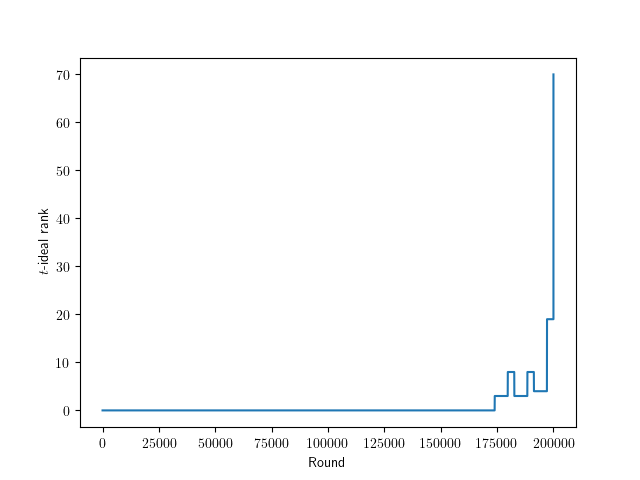
\includegraphics[width=0.9\textwidth]{honest_70_t_ideal.png}
        \caption{$t$-ideal rank evolution with 270 honest players, 70 posts and
        200.000 rounds}
        \label{fig:honest:70:tideal}
      \end{figure}

      \begin{figure}[!htbp]
        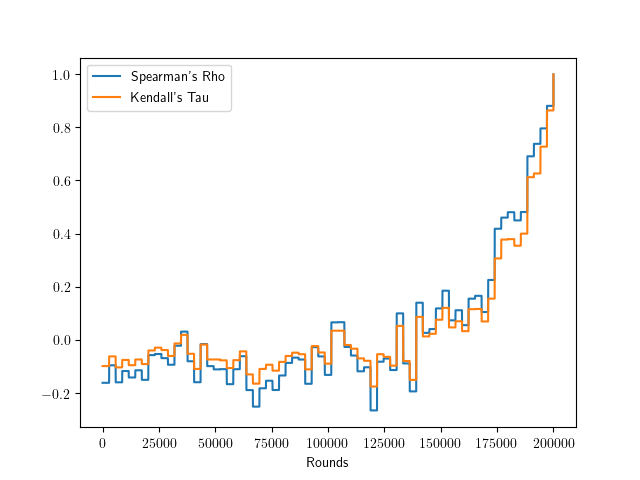
\includegraphics[width=0.9\textwidth]{honest_70_coeffs.png}
        \caption{Kendall's Tau and Spearman's Rho evolution with 270 honest
        players, 70 posts and 200.000 rounds}
        \label{fig:honest:70:coeffs}
      \end{figure}

      As we can see, both measures show that the real list converges rapidly to
      the ideal order at the very end of the execution; in the meanwhile, the
      quality of the list improves very slowly.

      Figures~\ref{fig:honest:100:tideal} and~\ref{fig:honest:100:coeffs} depict
      what happens when the rounds are not sufficient for all votes to be cast
      with full voting power. In particular, the corresponding simulation was
      executed with the same parameters as before, only changing $\postlen$ to
      100 and $\playerlen$ to 300. (Observe that $\rounds - 1 < \left(\postlen -
      1\right)\ceil*{\frac{a + b}{\regen}}$.)

      \begin{figure}[!htbp]
        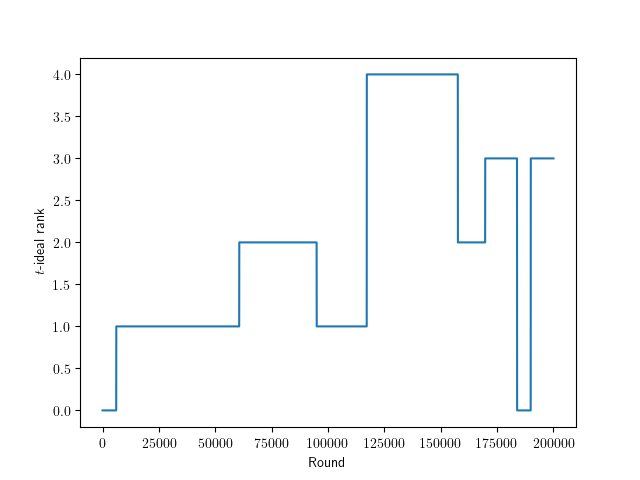
\includegraphics[width=0.9\textwidth]{honest_100_t_ideal.png}
        \caption{$t$-ideal rank evolution with 300 honest players, 100 posts and
        200.000 rounds}
        \label{fig:honest:100:tideal}
      \end{figure}

      \begin{figure}[!htbp]
        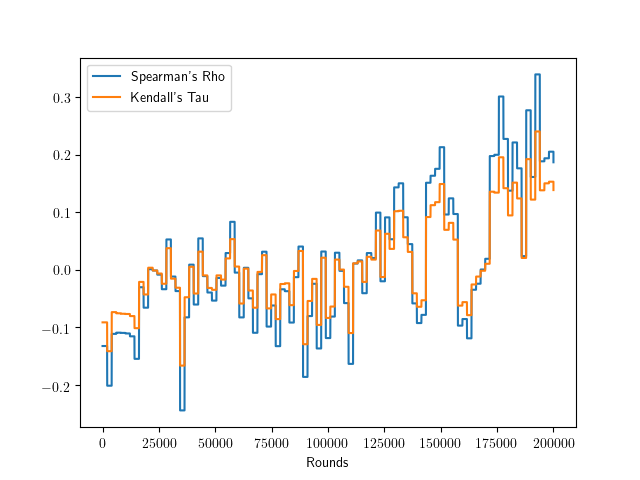
\includegraphics[width=0.9\textwidth]{honest_100_coeffs.png}
        \caption{Kendall's Tau and Spearman's Rho evolution with 300 honest
        players, 100 posts and 200.000 rounds}
        \label{fig:honest:100:coeffs}
      \end{figure}

      Here we see that at the end of the execution, only the first three posts
      are correctly ordered. Regarding the rest of the list, both Kendall's Tau
      and Spearman's Rho coefficients show that the order of the posts improves
      only slightly throughout the execution of the simulation.

    \subsubsection{Scenario B: Selfish users.}
      In order to understand how the presence of voting rings/Sybil accounts
      affects the curation quality, we simulate the execution of the game for
      various voting ring sizes. We fix the rest of the system parameters so
      that the selfish post is handicapped. In particular, the voting rounds are
      sufficient for all votes to be cast with full voting power, the likability
      of the selfish post is 0 for all players and it is initially placed at the
      bottom of the post list. Define the gain of the post of the selfish
      players as its ideal position minus its final position.
      Figure~\ref{fig:selfish:gain} depicts the gain of the selfish post for a
      varying number of selfish players, from 1 to 100.
      Figure~\ref{fig:selfish:tideal} shows the $t$-ideal rank of the resulting
      list at the same executions. For these simulations, the system parameters
      are $\playerlen = 101 .. 200, a = \frac{1}{50}, b = 10^{-4}, \regen =
      \frac{3}{5 \cdot 24 \cdot 60}, \attspan = 10, \rounds = 5000$.

      \begin{figure}[!htbp]
        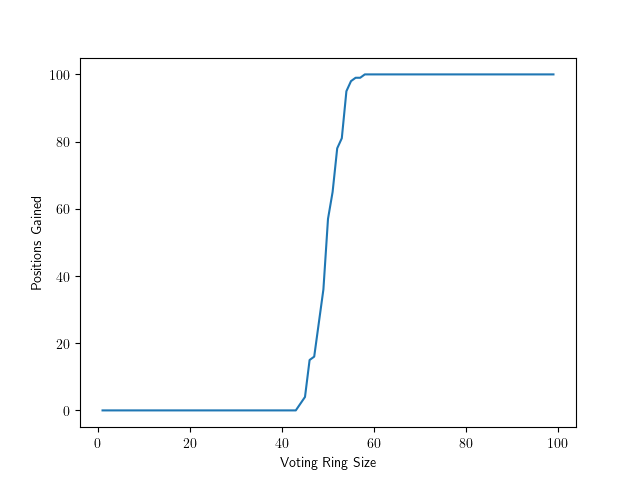
\includegraphics[width=0.9\textwidth]{selfish_positionsgained}
        \caption{Positions gained by selfish post with 100 honest players, 100
        posts and 1 to 100 selfish players}
        \label{fig:selfish:gain}
      \end{figure}

      \begin{figure}[!htbp]
        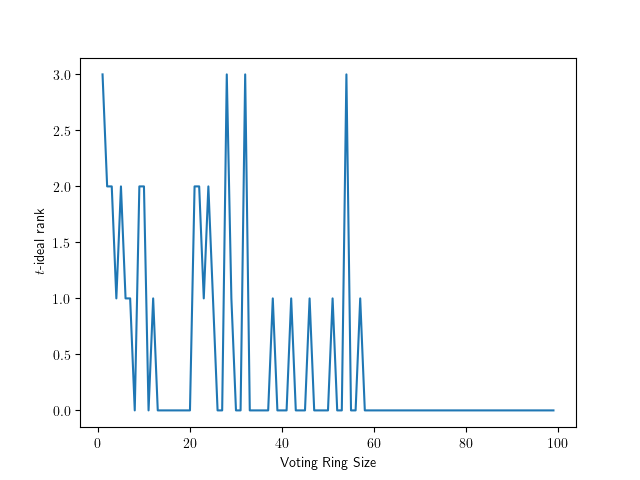
\includegraphics[width=0.9\textwidth]{selfish_t_ideal}
        \caption{$t$-ideal rank with 100 honest players, 100 posts and 1 to 100
        selfish players}
        \label{fig:selfish:tideal}
      \end{figure}
